%%%%%%%%%%%%%%%%%%%%%%%%%%%%%%%%%%%%%%%%%
% Short Sectioned Assignment
% LaTeX Template
% Version 1.0 (5/5/12)
%
% This template has been downloaded from:
% http://www.LaTeXTemplates.com
%
% Original author:
% Frits Wenneker (http://www.howtotex.com)
%
% License:
% CC BY-NC-SA 3.0 (http://creativecommons.org/licenses/by-nc-sa/3.0/)
%
%%%%%%%%%%%%%%%%%%%%%%%%%%%%%%%%%%%%%%%%%

%----------------------------------------------------------------------------------------
%	PACKAGES AND OTHER DOCUMENT CONFIGURATIONS
%----------------------------------------------------------------------------------------

\documentclass[paper=a4, fontsize=11pt]{scrartcl} % A4 paper and 11pt font size

\usepackage[T1]{fontenc} % Use 8-bit encoding that has 256 glyphs
\usepackage{fourier} % Use the Adobe Utopia font for the document - comment this line to return to the LaTeX default
\usepackage[spanish]{babel} % English language/hyphenation
\selectlanguage{spanish}
\usepackage[utf8]{inputenc}
\usepackage{amsmath,amsfonts,amsthm} % Math packages
\usepackage{graphicx}

\usepackage{sectsty} % Allows customizing section commands
\allsectionsfont{\centering \normalfont\scshape} % Make all sections centered, the default font and small caps

\usepackage{fancyhdr} % Custom headers and footers
\pagestyle{fancyplain} % Makes all pages in the document conform to the custom headers and footers
\date{}
\fancyhead{} % No page header - if you want one, create it in the same way as the footers below
\fancyfoot[L]{} % Empty left footer
\fancyfoot[C]{} % Empty center footer
\fancyfoot[R]{\thepage} % Page numbering for right footer
\renewcommand{\headrulewidth}{0pt} % Remove header underlines
\renewcommand{\footrulewidth}{0pt} % Remove footer underlines
\setlength{\headheight}{5.6pt} % Customize the height of the header

\numberwithin{equation}{section} % Number equations within sections (i.e. 1.1, 1.2, 2.1, 2.2 instead of 1, 2, 3, 4)
\numberwithin{figure}{section} % Number figures within sections (i.e. 1.1, 1.2, 2.1, 2.2 instead of 1, 2, 3, 4)
\numberwithin{table}{section} % Number tables within sections (i.e. 1.1, 1.2, 2.1, 2.2 instead of 1, 2, 3, 4)

\setlength\parindent{0pt} % Removes all indentation from paragraphs - comment this line for an assignment with lots of text

%----------------------------------------------------------------------------------------
%	TITLE SECTION
%----------------------------------------------------------------------------------------

\newcommand{\horrule}[1]{\rule{\linewidth}{#1}} % Create horizontal rule command with 1 argument of height

\title{	
\normalfont \normalsize 
\textsc{UNIVERSIDAD DE CANTABRIA, DEPARTAMENTO DE FÍSICA MODERNA} \\ [20pt] % Your university, school and/or department name(s)
\horrule{0.5pt} \\[0.4cm] % Thin top horizontal rule
\huge Física de Partículas Elementales (G71) \\ % The assignment title
\normalsize 4 Curso - Grado de Física - Doble Grado Física Matemáticas - Ejercicios Tema 1
\horrule{2pt} \\[0.5cm] % Thick bottom horizontal rule
}

\begin{document}

\maketitle % Print the title

\vspace{-2.5cm}

%----------------------------------------------------------------------------------------
%	PROBLEM 1
%----------------------------------------------------------------------------------------
\textbf{Cuestión 1.} Una partícual de masa 3 GeV viaja en la dirección positiva del eje Z con momento 4 GeV. ¿Cuál es su energía y su velocidad?
\\
\\
%----------------------------------------------------------------------------------------
%       PROBLEM 2
%----------------------------------------------------------------------------------------
\textbf{Cuestión 2.} Para un decaimiento $a\rightarrow 1 + 2$, muestra que la masa de la partícula a puede ser expresada como:
\begin{equation*}
m_{a}^2 = m_1^2 + m_2^2 + 2E_1E_2(1-\beta_1\beta_2cos(\theta))
\end{equation*}
\\
\\
%----------------------------------------------------------------------------------------
%       PROBLEM 3
%----------------------------------------------------------------------------------------
\textbf{Cuestión 3.} En el sistema de referencia de laboratorio, un protón con una energía total E colision con otro protón en reposo. Encuentra la energía mínima del proceso para
que el siguiente proceso esté cinemáticamente permitido.
\begin{equation*}
p + p \rightarrow p + p + \bar{p} + p
\end{equation*}
\\
\\
%----------------------------------------------------------------------------------------
%       PROBLEM 4
%----------------------------------------------------------------------------------------
\textbf{Cuestión 4.} Para el proceso $1 + 2 \rightarrow 3 + 4$, las variables de Mandelstam s, t y u, están definidas como $s = (p_1+p_2)^2$, $t = (p_1-p_3)^2$ y $u = (p_1-p_4)^2$. Demuestra que:
\begin{equation*}
s + u + t = m_1^2 + m_2^2 + m_3^2 + m_4^2
\end{equation*}
\\
\\
%----------------------------------------------------------------------------------------
%       PROBLEM 5
%----------------------------------------------------------------------------------------
\textbf{Cuestión 5.} En un experimento de blanco fijo protón-protón, ¿Qué relación guarda el llamado flujo invariante Lorentz con la sección eficaz?. \textbf{(0.5 puntos)}. Calcula el valor del flujo invariante Lorentz
$F=4[(p^\mu_1p_{2\mu})^2 - m_1^2 m_2^2]^{1/2}$ para el caso en el que la partícula 1 tiene momento $\vec{p}_1$ y la partícula 2 está en reposo. \textbf{(1 punto)}. ¿Por qué
con frecuencia se da la sección eficaz diferencial en términos de $\frac{d\sigma}{dt}$ donde t es el invariante de Mandelstam?. ¿Qué ventajas aporta esto en el contexto
de la comparación de resultados en diferentes experimentos?. Razona tu respuesta. \textbf{(0.5 puntos)}. 
  
\vspace{3cm}

\begin{figure}[!h]
\begin{center}
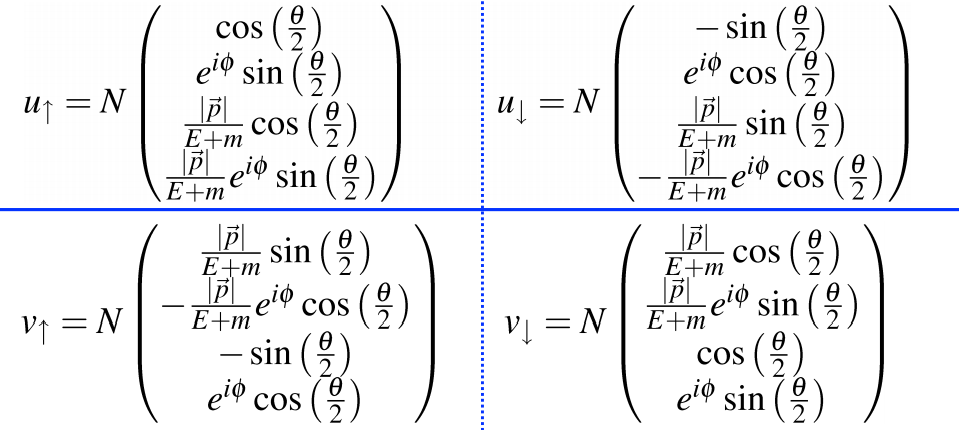
\includegraphics[width=0.6\linewidth]{espinores.png}
\end{center}
\caption{Espinores solución a la ecuación de Dirac y autoestados del operador helicidad.}
\label{espinores}
\end{figure}


\begin{figure}[!h]
\begin{center}
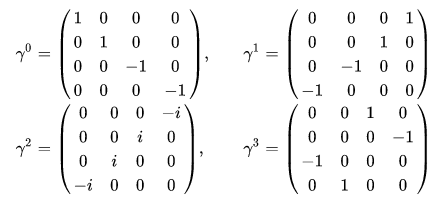
\includegraphics[width=0.6\linewidth]{matrices.png}
\end{center}
\caption{Matrices de Dirac.}
\label{matrices}
\end{figure}






\end{document}
